\documentclass[11pt]{article}
\usepackage{tocloft}
\usepackage{graphicx}
\usepackage{calc}
\usepackage{amssymb}
\usepackage{color}
\usepackage{array}
\usepackage[sc]{mathpazo}
\usepackage{url}
\usepackage[final]{pdfpages}
\usepackage{amsmath}

%\linespread{1.05}
\oddsidemargin=0pt
\evensidemargin=0pt
\textwidth=6.5in
\topmargin=0pt
\headheight=0pt
\headsep=0pt
\textheight=9in
% EXPERIMENTAL
%\parindent=0pt
%\parskip=3pt
\setlength{\parindent}{0cm}
\newcommand\secfont{\fontfamily{cmss}\selectfont}%\textwidth 5.5truein
\newcommand\pifheading[1]{{\secfont\textbf{#1}:}}
%\oddsidemargin -0.40truein
%\textheight 8.0truein
%\topmargin -0.25truein
\def\lo{
\mathrel{\raise.3ex\hbox{$<$}\mkern-14mu\lower0.6ex\hbox{$\sim$}}
}
\def\hi{
\mathrel{\raise.3ex\hbox{$>$}\mkern-14mu\lower0.6ex\hbox{$\sim$}}
}

\textwidth = 6.6 in
\textheight = 9.1 in
\oddsidemargin = -0.05 in
\evensidemargin = +0.05 in
\topmargin = -.1 in
\headheight = 0.0 in
\headsep = 0.0 in
\parskip = 0.06in
\newcommand\registered{{\ooalign{\hfil\raise .00ex\hbox{\scriptsize R}\hfil\crcr\mathhexbox20D}}}

%% Define a new 'leo' style for the package that will use a smaller font.
\makeatletter
\def\url@leostyle{%
  \@ifundefined{selectfont}{\def\UrlFont{\sf}}{\def\UrlFont{\small\ttfamily}}}
\makeatother
%% Now actually use the newly defined style.
\urlstyle{leostyle}

%\pagestyle{empty}
%\includeonly{previous,proposal_references}
%\includeonly{proposal_references}
%\includeonly{previous}

% TOC

\begin{document}
%%%%%%%%%%%%%%%%%%%%%%%%%%%%%%%%%%%%%%%%%%%%%%%%%%%%%%%%%%%%%%%%%%%%%
\begin{center}
\textbf{\Large
AST101: Our Corner of the Universe \\
\vspace*{0.1cm}
Lab 3: The Phases of the Moon
}
\end{center}

\vspace*{0.5cm}

{\Large Name:}\vspace*{0.5cm}\\\hrule
{\Large Student number (SUID):}\vspace*{0.5cm}\\\hrule
{\Large Lab section:}\vspace*{0.5cm}\\\hrule
{\Large Group Members:}\vspace*{0.5cm}\\\hrule
\vspace*{0.5cm}

%%%%%%%%%%%%%%%%%%%%%%%%%%%%%%%%%%%%%%%%%%%%%%%%%%%%%%%%%%%%%%%%%%%%%
\section{Introduction}

Last week, we studied the Sun, at great length. This week, we turn our attention to the next most prominent celestial object in our sky; the Moon. Unlike many of the objects we see, the Moon appears to change both its location and its nature, appearing at times as a tiny sliver and at others as a filled circle, and everything in between. Ancient societies used this transient nature of the Moon to mark the passage of time in their calendars, and to denote the beginning of special festivals. Our own Gregorian calendar has a remnant of this: our months are approximations of the lunar cycle. We will study the Moon, and the cause for its phases, in detail today. 

This lab will involve extensive drawing of your own diagrams. Take this seriously and make sure you understand it;
you will need this skill for Exam 1.

\subsection*{Materials}

We will once again be using Stellarium. 

\subsection*{Objective}

To catalog the phases of the Moon, and understand their cause.

\newpage

\section{Cataloging The Moon Phases}

\subsection{Observing a Moon Phase}

Depending on when you look at it, the Moon can either appear as a tiny sliver of light, a semi-circle of light, an almost full circle of light, and an actually full circle of light. These different appearances of the Moon are called the \textbf{phases of the Moon}.

\noindent
\textbf{Question 1.} Turn on Stellarium, set your location to Syracuse New York, and the date to September 14 2019. Open up the search box, and use it to find the Moon. (If you can't see the Moon, advance time slowly forward until you see it in the sky. You should be able to see the Moon during most of the night on this day.)

Once you're looking at the Moon, zoom in until you can clearly see its surface.\\

Describe the bright part of the Moon, specifically commenting on its shape, location, and size (How much of the Moon's visible surface does it take up?).\\
\vspace*{1.5cm}

\hrulefill\\
\noindent

\textbf{Question 2.} On the blank circle below, sketch the appearance of the Moon by shading in the dark parts and leaving the lit parts unshaded. Do not worry about drawing the details of the surface, just what is lit and what is not. This is the \textbf{full moon} phase of the Moon.\\
\begin{center}
	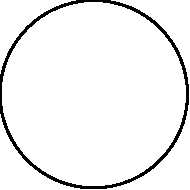
\includegraphics{blank_moon}
\end{center}

\newpage


Page 11 of your lab handout is a drawing of the Moon's orbit around the Earth. The position 
of the full moon is already drawn for you. (Label it ``full moon'' along with the date, 13 September.) The right half of the Moon's surface is shaded, since it is pointed away from the Sun and thus not illuminated.

Turn to this page and tear it out (along with Page 9, which you will use later); you'll add things to it as you go.\vspace{1cm}

\textbf{Question 3.} Which portion of the Moon is pointed toward Earth? Shade the half of the Moon that you {\it can't}
see because it is pointed away from Earth with your pencil, and use a highlighter to highlight the half that you {\it can} see.

Now, consider only the portion you've highlighted -- the part that is pointed toward Earth. What fraction of it is lit 
by the Sun? Does this match what you see in Stellarium?

\vspace*{1.5cm}

\hrulefill\\

\textbf{Question 4.} What time of day is this moon highest in the sky? Check with Stellarium: does this match your 
prediction from the drawing? Add this information next to the full moon.

\vspace*{1.5cm}

\hrulefill\\

\textbf{Question 5.} How far will the Moon have traveled around the Earth in four hours? Predict how the Moon's phase and position
in the sky will change during this time. 

\vspace*{1.5cm}

\hrulefill\\


\subsection{Touring the Phases}


We'll now follow the Moon during half of its cycle to see how its phase changes, and how you can predict its phase from your drawing.

It takes the Moon about 29 days to go through a cycle of phases. Since the phases are caused by the Moon's motion around the Earth,
this means that it travels halfway around the Earth in about 14 days, a quarter of the way around the Earth in about 7 days, and one-eighth of the way around the Earth in about 3-4 days.

Draw circles corresponding to the Moon's position on your diagram for September 17, September 20, September 24, and September 27. In the next few exercises, you'll determine what phases of the moon these correspond to.

\newpage

For the next phase (September 17), we'll need to think a little harder to figure out what phase the Moon will be on this date. 
To do this, follow this procedure:

\begin{enumerate}
	\item Shade in the portion of the Moon (using horizontal lines) that isn't lit by the Sun. (This will always be the right half in this picture.) This is the portion of the Moon that we can't see because it isn't giving off any light.
	\item Draw a line from the center of the Earth to the center of the Moon. This represents the sight line from the Earth to the Moon.
	\item Then, draw a line that goes through the center of the Moon that is perpendicular to the sight line. This is called the ``perpendicular bisector'', and separates the portion of the Moon we can see (the front half) from the portion that we can't (the back half).
	\item Shade the half of the Moon that we can't see with vertical lines, then use your yellow highlighter to highlight the half of the Moon that we can see.
\end{enumerate}

\textbf{Question 6.} What fraction of the visible part of the Moon (the highlighted part) is lit by the Sun (not shaded in)? What do you expect this phase of the Moon to look like?


\vspace*{1.5cm}

\hrulefill\\

\textbf{Question 7.} Now use Stellarium to confirm your prediction. Draw the phase of the Moon below. This phase is called ``waning gibbous''. ``Waning'' means ``getting less full'', and ``gibbous'' comes from an old word meaning ``fat'', i.e. still mostly full. (The Moon is waning now, since it is less full than it was four days ago.)
Draw the phase that you see on the bottom of the back page.


\textbf{Question 8.} At what time do you expect this moon phase (approximately) to be highest in the sky? Write down your prediction on the diagram. (If you're not completely sure, go check in Stellarium, but you shouldn't need to!)

\vspace*{1.5cm}

\hrulefill\\
\newpage

\textbf{Question 9.} Repeat the previous for the next three positions of the Moon: September 20, September 24, and September 27. 
For each one, follow the procedure on the previous page (drawing on your page) to predict what the moon phase on that date will look like.
If you're not sure, check in Stellarium. The three phases you will see (not in order) are:

\begin{itemize}
	\item New moon: {\it none} of the Moon visible from Earth is lit by the Sun
	\item Waning crescent: Less than half of the Moon visible from the Earth is lit by the Sun, and every day the visible portion is becoming smaller
	\item Waning half moon: About half of the Moon visible from the Earth is lit by the Sun, and every day the visible portion is becoming smaller
\end{itemize}

Add these three phases to the information on the last page. Label what they are, draw what they look like from Earth, and 
estimate what time they'll be highest in the sky.

\vspace{1in}

\textbf{Question 10.} You've only done half of a lunar cycle, but you should be able to guess what happens during the other half.
You don't need to do the entire perpendicular bisector procedure, but you should be able to guess the position of the Moon on 
October 1, October 4, and October 8, along with its phase. Since the Moon is becoming gradually more full during this period, 
the phases here are called ``waxing'': waxing crescent, waxing half, waxing gibbous. Label their positions in the Moon's orbit (on the bottom half), and draw them below.

\newpage

\section{Rising and Setting}

Recall that, as seen from above the North Pole:

\begin{itemize}
	\item The Earth rotates on its axis counterclockwise once in 24 hours
	\item The Moon revolves counterclockwise around the Earth once in 29 days\footnote{This is a little bit of a fudge -- if you're curious, read about the difference between the {\it sidereal period} of the Moon and the {\it synodic period}.}
	\item {\it East} is the side of the horizon that things rise (that is, appear) over; {\it West} is the side of the horizon that things set (that is, disappear) under. East is not necessarily on the right, and West is not necessarily on the left; these are totally arbitrary features of maps drawn by Europeans from the modern era.
\end{itemize}


\textbf{Question 11.} Look at the diagram on page 9. (Tear that one off as well if you have not already.) During the Earth's rotation in one day, an observer will pass through each of the positions shown. Label each one with the time of day that it represents.

\textbf{Question 12.} Get a blank piece of paper to serve as the horizon. Hold the paper vertically so that it passes through the center of the Earth, obscuring the left half of the diagram. Rotate this piece of paper counterclockwise to represent the passage of time, and notice that at some point the Moon will appear above the horizon. Label the side of the horizon that the Moon has appeared over ``East''; the other side is ``West''.

\textbf{Question 13.} When the horizon is in this position, what time is it? (Remember that the horizon is parallel to the observer's feet, separating the world below their feet that they can't see from the world above their head that they can.) This is the time that the moon phase shown will rise above the eastern horizon.

\vspace*{1.5cm}

\hrulefill\\
\newpage

\textbf{Question 14.} By rotating the horizon, you can determine where the Sun and Moon will appear in the sky at any time of day. Fill out the following table using your diagram and your ``horizon'', using the following options:


\begin{itemize}
	\item Below the horizon (not visible)
	\item Just rising in the East
	\item In the eastern sky
	\item Nearly overhead
	\item In the western sky
	\item Just setting in the West
\end{itemize}
\Large
\begin{tabular}{|c|c|c|}
\hline 

Time & Position of Sun & Position of Moon \\ \hline
Midnight & & \\ \hline
3:00 AM & & \\ \hline
6:00 AM & & \\ \hline
9:00 AM & & \\ \hline
Noon   & & \\ \hline
3:00 PM & & \\ \hline
6:00 PM & & \\ \hline
9:00 PM & & \\ \hline
\end{tabular}
\normalsize
\vspace{1.5cm}

\textbf{Question 15.} Putting everything together and looking at the two diagrams you've completed, figure out what time of day a {\it waning gibbous} moon will be setting in the west. If you can do this, you're well-equipped to handle any question I might ask about the Moon on Exam 1!

\vspace{1.5in}

\textbf{Question 16.} Ask your TA to look at your diagrams if you've not already, and discuss anything you're not sure about with them.
They should initial below that you've completed them. You may take your diagrams home with you to remind you how this works, and to help you
study for Exam 1.

\newpage
\begin{center}
	(This page left blank)
\end{center}

\newpage

\begin{center}
	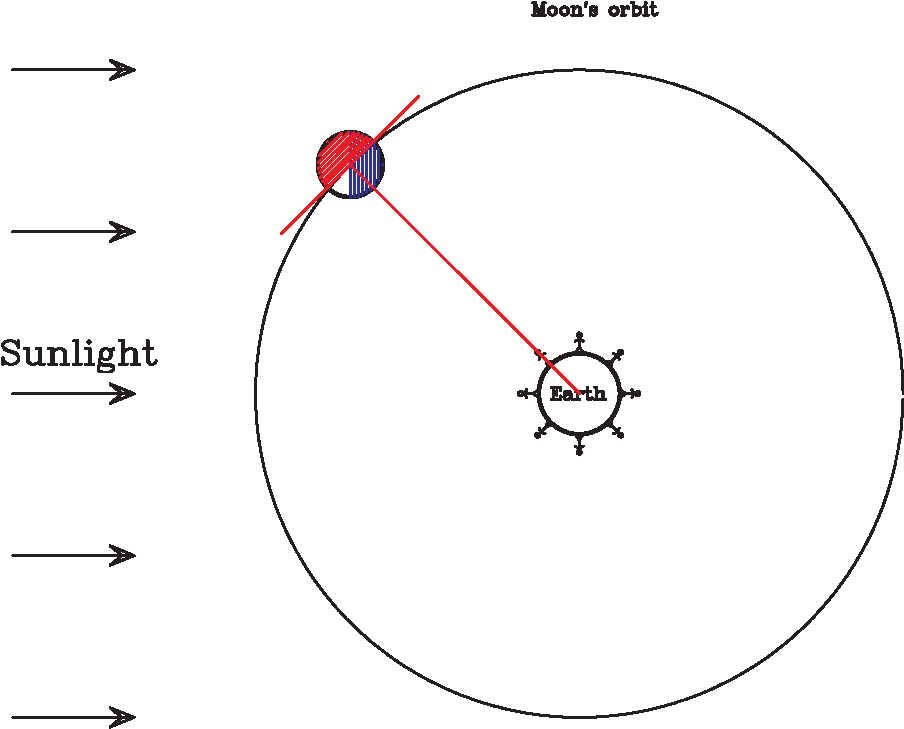
\includegraphics[width=0.8\textwidth]{allpositions-crop.pdf}
\end{center}

\newpage
\begin{center}
(This page left blank)
\end{center}

\newpage

You should tear this diagram out and fill it out as you go. You should eventually label five positions (along the top half of the Moon's orbit)
with the phase of the moon, the date on which it occurs, and the time of day that it will be highest in the sky.

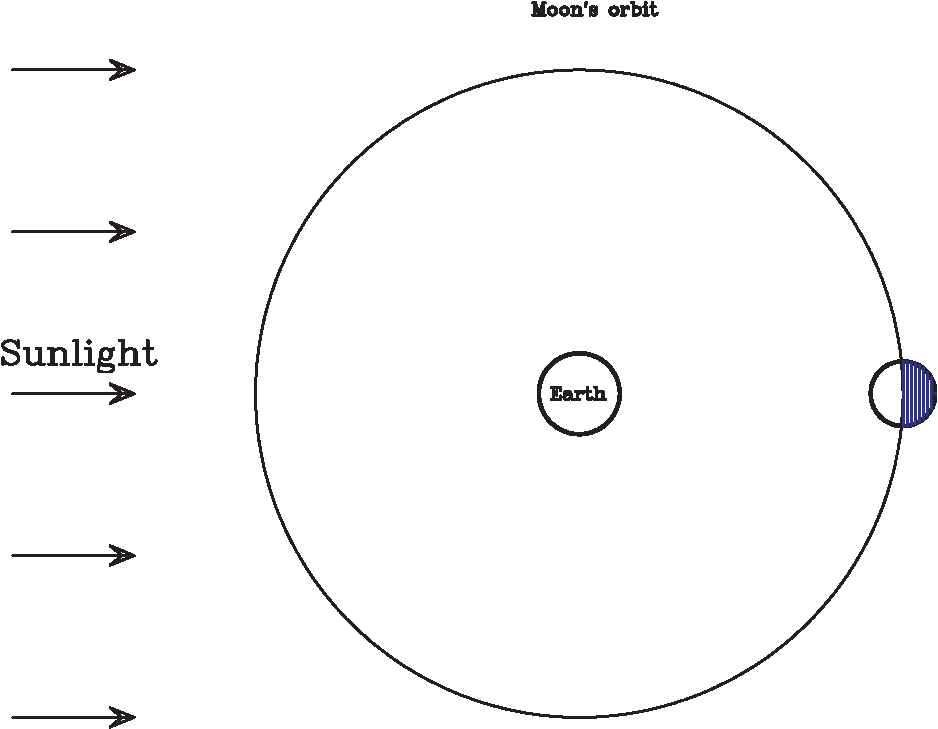
\includegraphics[width=0.9\textwidth]{moon-diagram-full-shade-crop.pdf}

Below, sketch the Moon phase as it appears on the given date.\\
\begin{align*}
& \ \ \ \ 9/14 & 
& \ \ \ \ 9/18 &
& \ \ \ \ 9/21 &
& \ \ \ \ 9/25 & 
& \ \ \ \ 9/28 &
& \ \ \ \ 10/2 &
& \ \ \ \ 10/5 &
& \ \ \ \ 10/9\\
& 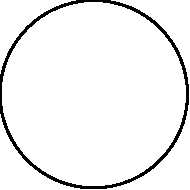
\includegraphics[scale=0.55]{blank_moon} &
& 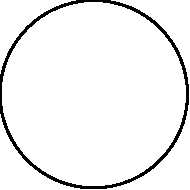
\includegraphics[scale=0.55]{blank_moon} &
& 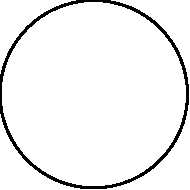
\includegraphics[scale=0.55]{blank_moon} &
& 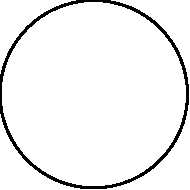
\includegraphics[scale=0.55]{blank_moon} &
& 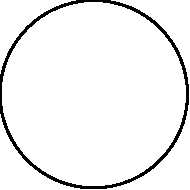
\includegraphics[scale=0.55]{blank_moon} &
& 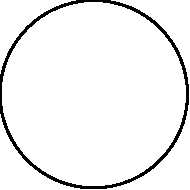
\includegraphics[scale=0.55]{blank_moon} &
& 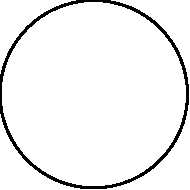
\includegraphics[scale=0.55]{blank_moon} &
& 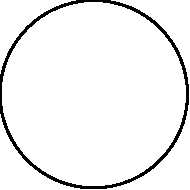
\includegraphics[scale=0.55]{blank_moon} & 
& 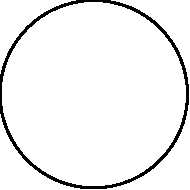
\includegraphics[scale=0.55]{blank_moon} &
\end{align*}


\end{document}
